%  The AAU Poster Theme.
%  2013-05-08 v. 1.1.0
%  Copyright 2013 by Jesper Kjær Nielsen <jkn@es.aau.dk>
%
%  This is free software: you can redistribute it and/or modify
%  it under the terms of the GNU General Public License as published by
%  the Free Software Foundation, either version 3 of the License, or
%  (at your option) any later version.
%
%  This is distributed in the hope that it will be useful,
%  but WITHOUT ANY WARRANTY; without even the implied warranty of
%  MERCHANTABILITY or FITNESS FOR A PARTICULAR PURPOSE.  See the
%  GNU General Public License for more details.
%
%  You can find the GNU General Public License at <http://www.gnu.org/licenses/>.
\documentclass[a0paper,portrait]{baposter}
%%%%%%%%%%%%%%%%%%%%%%%%%%%%%%%%%%%%%%%%%%%%%%%%
% Language, Encoding and Fonts
% http://en.wikibooks.org/wiki/LaTeX/Internationalization
%%%%%%%%%%%%%%%%%%%%%%%%%%%%%%%%%%%%%%%%%%%%%%%%
% Select encoding of your inputs. Depends on
% your operating system and its default input
% encoding. Typically, you should use
%   Linux  : utf8 (most modern Linux distributions)
%            latin1 
%   Windows: ansinew
%            latin1 (works in most cases)
%   Mac    : applemac
% Notice that you can manually change the input
% encoding of your files by selecting "save as"
% an select the desired input encoding. 
\usepackage[utf8]{inputenc}
% Make latex understand and use the typographic
% rules of the language used in the document.
\usepackage[english]{babel}
% Use the vector font Latin Modern which is going
% to be the default font in latex in the future.
\usepackage{helvet}
% Change the default font family from roman to sans serif
\renewcommand{\familydefault}{\sfdefault} % for text
\usepackage[helvet]{sfmath} % for math
% Choose the font encoding
\usepackage[T1]{fontenc}
% Prevent hyphenation
\usepackage[none]{hyphenat}

%%%%%%%%%%%%%%%%%%%%%%%%%%%%%%%%%%%%%%%%%%%%%%%%
% Graphics and Tables
% http://en.wikibooks.org/wiki/LaTeX/Importing_Graphics
% http://en.wikibooks.org/wiki/LaTeX/Tables
% http://pgfplots.sourceforge.net/ 
%%%%%%%%%%%%%%%%%%%%%%%%%%%%%%%%%%%%%%%%%%%%%%%%
% You cannot use floats in the baposter theme.
% We therefore load the caption package which provides
% the command \captionof
% Set up how figure and table captions are displayed
\usepackage{caption}
\captionsetup{
  font=small,% set font size to footnotesize
  labelfont=bf % bold label (e.g., Figure 3.2) font
}
% Make the standard latex tables look so much better
\usepackage{array,booktabs}
% For creating beautiful plots
\usepackage{pgfplots}
\graphicspath{{./figures/}}
% Document-style algorithms
\usepackage[ruled,vlined,linesnumbered]{algorithm2e}
\SetKwInOut{Input}{input}
\SetKwInOut{Output}{output}

%%%%%%%%%%%%%%%%%%%%%%%%%%%%%%%%%%%%%%%%%%%%%%%%
% Mathematics
% http://en.wikibooks.org/wiki/LaTeX/Mathematics
%%%%%%%%%%%%%%%%%%%%%%%%%%%%%%%%%%%%%%%%%%%%%%%%
% Defines new environments such as equation,
% align and split 
\usepackage{amsmath}
% Adds new math symbols
\usepackage{amssymb}
\usepackage{mathrsfs}

%%%%%%%%%%%%%%%%%%%%%%%%%%%%%%%%%%%%%%%%%%%%%%%%
% Colours
% http://en.wikibooks.org/wiki/LaTeX/Colors
%%%%%%%%%%%%%%%%%%%%%%%%%%%%%%%%%%%%%%%%%%%%%%%%
\selectcolormodel{RGB}
% define the three aau colors
\definecolor{aaublue1}{RGB}{68,84,106}% dark blue
\definecolor{aaublue2}{RGB}{113,109,143} % light blue
\definecolor{aaublue3}{RGB}{160,170,175} % lighter blue

%%%%%%%%%%%%%%%%%%%%%%%%%%%%%%%%%%%%%%%%%%%%%%%%
% Lists
% http://en.wikibooks.org/wiki/LaTeX/List_Structures
%%%%%%%%%%%%%%%%%%%%%%%%%%%%%%%%%%%%%%%%%%%%%%%%
% Easier configuration of lists
\usepackage{enumitem}
%configure itemize
\setlist{%
  topsep=0pt,% set space before and after list
  noitemsep,% remove space between items
  labelindent=\parindent,% set the label indentation to the paragraph indentation
  leftmargin=*,% remove the left margin
  font=\color{aaublue1}\normalfont, %set the colour of all bullets, numbers and descriptions to aaublue1
}
% use set<itemize,enumerate,description> if you have an older latex distribution
\setitemize[1]{label={\raise1.25pt\hbox{$\blacktriangleright$}}}
\setitemize[2]{label={\scriptsize\raise1.25pt\hbox{$\blacktriangleright$}}}
\setitemize[3]{label={\raise1.25pt\hbox{$\star$}}}
\setitemize[4]{label={-}}
%\setenumerate[1]{label={\theenumi.}}
%\setenumerate[2]{label={(\theenumii)}}
%\setenumerate[3]{label={\theenumiii.}}
%\setenumerate[4]{label={\theenumiv.}}
%\setdescription{font=\color{aaublue1}\normalfont\bfseries}

% use setlist[<itemize,enumerate,description>,<level>] if you have a newer latex distribution
%\setlist[itemize,1]{label={\raise1.25pt\hbox{$\blacktriangleright$}}}
%\setlist[itemize,2]{label={\scriptsize\raise1.25pt\hbox{$\blacktriangleright$}}}
%\setlist[itemize,3]{label={\raise1.25pt\hbox{$\star$}}}
%\setlist[itemize,4]{label={-}}
%\setlist[enumerate,1]{label={\theenumi.}}
%\setlist[enumerate,2]{label={(\theenumii)}}
%\setlist[enumerate,3]{label={\theenumiii.}}
%\setlist[enumerate,4]{label={\theenumiv.}}
%\setlist[description]{font=\color{aaublue1}\normalfont\bfseries}

%%%%%%%%%%%%%%%%%%%%%%%%%%%%%%%%%%%%%%%%%%%%%%%%
% Misc
%%%%%%%%%%%%%%%%%%%%%%%%%%%%%%%%%%%%%%%%%%%%%%%%
% change/remove some names
\addto{\captionsenglish}{
  %remove the title of the bibliograhpy
  \renewcommand{\refname}{\vspace{-0.7em}}
  %change Figure to Fig. in figure captions
  \renewcommand{\figurename}{Fig.}
}
% create links
\usepackage{url}
%note that the hyperref package is currently incompatible with the baposter class

%%%%%%%%%%%%%%%%%%%%%%%%%%%%%%%%%%%%%%%%%%%%%%%%
% Macros
%%%%%%%%%%%%%%%%%%%%%%%%%%%%%%%%%%%%%%%%%%%%%%%%
\newcommand{\alert}[1]{{\color{aaublue1}#1}}




%%%%%%%%%%%%%%%%%%%%%%%%%%%%%%%%%%%%%%%%%%%%%%%%
% Document Start 
%%%%%%%%%%%%%%%%%%%%%%%%%%%%%%%%%%%%%%%%%%%%%%%%
\begin{document}
%%%%%%%%%%%%%%%%%%%%%%%%%%%%%%%%%%%%%%%%%%%%%%%%
% Some changes that cannot be made in the preamble
%%%%%%%%%%%%%%%%%%%%%%%%%%%%%%%%%%%%%%%%%%%%%%%%
% set the background of the poster
\background{
  \begin{tikzpicture}[remember picture,overlay]%
    %the poster background color
    \fill[fill=aaublue3] (current page.north west) rectangle (current page.south east);
    %the header
    \fill [fill=aaublue1] (current page.north west) rectangle ([yshift=-\headerheight] current page.north east);
  \end{tikzpicture}
}
% if you want to reduce the space before and after equations, use and adjust
% the following lines
%\addtolength{\abovedisplayskip}{-2mm}
%\addtolength{\belowdisplayskip}{-2mm}

%%%%%%%%%%%%%%%%%%%%%%%%%%%%%%%%%%%%%%%%%%%%%%%%
% General poster setup
%%%%%%%%%%%%%%%%%%%%%%%%%%%%%%%%%%%%%%%%%%%%%%%%
\begin{poster}{
  %general options for the poster
  grid=false,
  columns=3,
%  colspacing=4.2mm,
  headerheight=0.1\textheight,
  background=user,
%  bgColorOne=red!42, %is used when background != user and none
%  bgColortwo=green!42, %is used when background is shaded
  eyecatcher=false,
  %posterbox options
  headerborder=closed,
  borderColor=aaublue1,
  headershape=roundedright,
  headershade=plain,
  headerColorOne=aaublue1,
%  headerColortwo=yellow!42, %is used when the header background is shaded
  textborder=roundedleft,
  boxshade=plain,
  boxColorOne=white,
%  boxColorTwo=cyan!42,%is used when the text background is shaded
  headerFontColor=white,
  headerfont=\Large\sf\bf,
  linewidth=1pt
}
%the Eye Catcher (the logo on the left)
{
  %this can be commented out or replaced by a company/department logo
  
\includegraphics[height=0.75\headerheight]{logo_sorb}
}
%the poster title
{\color{white}\bf
  Lifelong Learning with \\Dynamically Expandable Networks
}
%the author(s)
{\color{white}\normalsize\\
  \textbf{Octave Mariotti \& Rémy Portelas,}\\ {ICLR Reproducibility Challenge 2018}\\
} % Je teste ce que j'avais en tete
%the logo (the logo on the right)
{
  %this can be commented out or replaced by a company/department logo
  
\includegraphics[height=0.75\headerheight]{logo_sorb}
}
























































%%%%%%%%%%%%%%%%%%%%%%%%%%%%%%%%%%%%%%%%%%%%%%%%
% the actual content of the poster begins here
%%%%%%%%%%%%%%%%%%%%%%%%%%%%%%%%%%%%%%%%%%%%%%%%

\begin{posterbox}[name=intro,column=0,row=0]{Context}

\textbf{Lifelong learning}\cite{LL94} is a learning paradigm in which the model must learn tasks one after the other and tries to transfer knowledge from old tasks to new ones. This incremental deep learning setting raises challenging problems both in terms of scalability and efficiency.\\

A \textbf{Dynamically Expandable Network} (DEN) is a novel deep architecture meant to address these issues\cite{DEN17}. The idea is to dynamically expand the network to learn a compact overlapping knowledge structure while limiting semantic drift.\\

In this review we will give an \textbf{in-depth description} of the authors' DEN model. We will then show \textbf{our results} obtained by reproducing their experiment on performance using a variation of the MNIST dataset. Finally, we will \textbf{discuss} the limitations of this paper.

\vspace{3pt}
\end{posterbox}

\begin{posterbox}[name=DEN,column=0,below=intro]{The DEN model}
The DEN model combines several ideas from the literature in order to create a learning procedure able to automatically accommodate new tasks by adding neurons while retaining knowledge from the previous ones.

\begin{algorithm}[H]
\small
\caption{Base DEN algorithm}
\Indm
\Input{Dataset $D = (D_1,…,D_T)$}
\Output{Network parameters $W_T$}
\Indp
    \For{t in 1,…,T}{
        \If{t == 1}{
            train network with $\ell_1$ regularization\;
        }
        \Else
        {
            $W_{sr}$ = \text{Selective\_retraining}($W_{t-1}$)\;
            \If{$\mathcal{L}>\tau$}{
            $W_{ne}$ = \text{Network\_expansion}($W_{sr}$)\;
            }{}
        $W_{t}$ = \text{Duplication}($W_{ne}$)\;
        }
    }
\end{algorithm}
\vspace{2pt}
\end{posterbox}



\begin{posterbox}[name=expe,column=0,below=DEN]{Experimental Reproduction}
Our experiments (box below on the right) show poor DEN performances along with unexpectedly high baselines, both averaged over five random splits.

Several discrepancies were observed between released code and the algorithm described in the article.
\vspace{3pt}
\end{posterbox}



\begin{posterbox}[name=archi,column=1,row=0,span=2]{DEN Architecture}
\begin{center}
    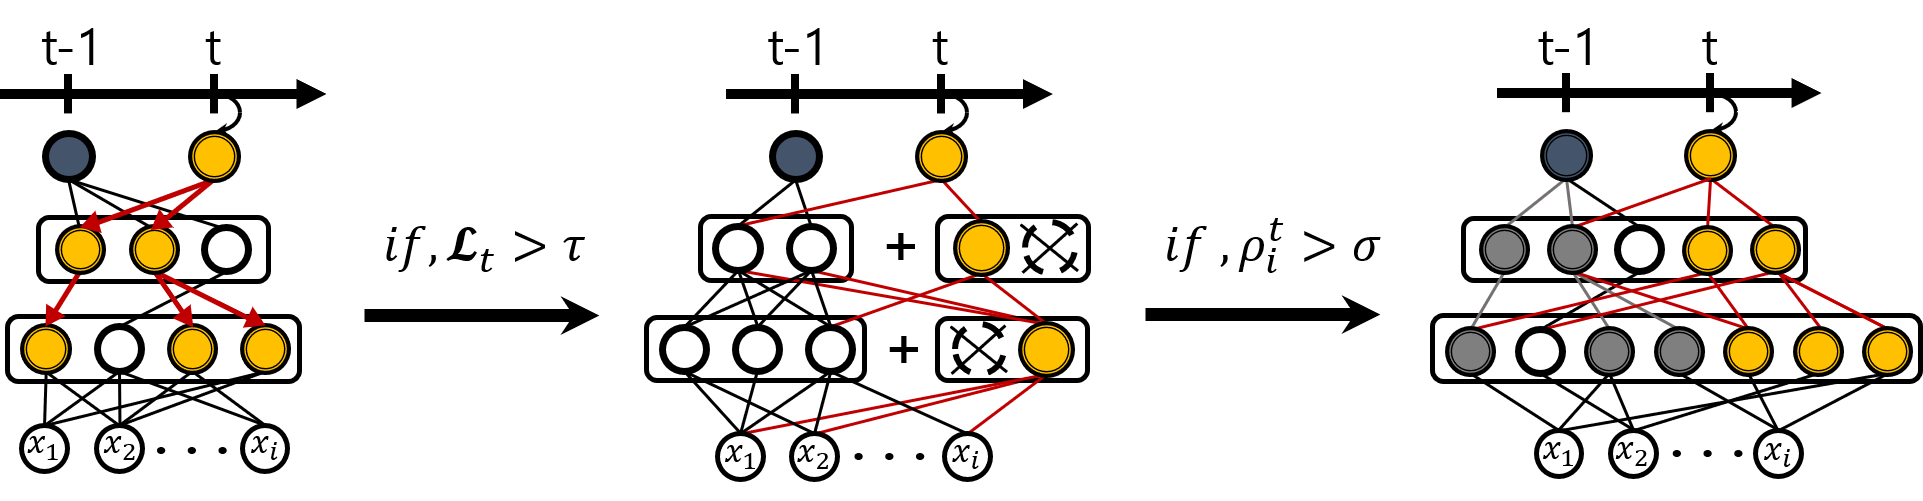
\includegraphics[width=\textwidth]{DEN_layout}
    \label{den_pipe}
\end{center}
\vspace{-25pt}
\small The 3 steps of a DEN: \textbf{Selective Retrain} (\textit{left}), \textbf{Dynamic Network Expansion} (\textit{middle}), \textbf{Duplication} (\textit{right}).
\end{posterbox}


\begin{posterbox}[name=SR,column=1,below=archi]{Selective retraining}
When a new tasks arrives, we want to learn it with the help of the knowledge from previous tasks. The \textbf{Selective retraining} algorithm is tasked with selecting neurons that are useful for this new task and training them.

\begin{algorithm}[H]
\small
\caption{Selective Retraining}
\Indm
\Input{Dataset $D_t$, previous parameters $W_{t-1}$}
\Output{Network parameters $W_{sr}$}
\Indp
    Retrain last layer only with $\ell_1$ regularization\;
    Perform breadth-first search in network to select useful neurons\;
    Train subnetwork with $\ell_2$ regularization\;
\end{algorithm}
\textcolor{black}{
Since the network is sparse, this algorithm only retrains neurons that are connected to the output neuron associated with the new task, preventing negative transfer.
}
\end{posterbox}



\begin{posterbox}[name=DNE,column=1,below=SR]{Dynamic Network Expansion}
If the loss is not low enough after \textbf{Selective Retraining}, then we must increase the network's size to improve our performances on the current task.

\begin{algorithm}[H]
\small
\caption{Dynamic Expansion}
\Indm
\Input{Dataset $D_t$,Loss $\mathcal{L}$}
\Output{Expanded Network $W_{ne}$}
\Indp
    \If {$\mathcal{L} > \tau$}{
        Add $k$ units $\textbf{h}^{\mathcal{N}}$ at all layers\;
        Train network with $\ell_1$ and $\ell_ {gs}$\;}
    \ForAll {layer l}{
        Remove useless units in $\textbf{h}^{\mathcal{N}}_l$\;}
\end{algorithm}
\textcolor{black}{
The combined use of $\ell_1$-norm and \textbf{group sparse regularization} $\ell_{gs}$ (a group being all incoming connections of a neuron) allows us to drop unnecessary neurons, effectively keeping the network both accurate and compact.
}
\end{posterbox}







\begin{posterbox}[name=dup,column=2,below=archi]{Duplication}
In lifelong learning, an important challenge is to prevent \textbf{catastrophic forgetting}, that is forgetting how to perform old tasks when learning new ones. The \textbf{duplication} algorithm selects neurons in the network that have changed from the last iteration and duplicates them in order to preserve performances on both the new and the old task.

\begin{algorithm}[H]
\small
\caption{Neuron Duplication}
\Indm
\Input{Dataset $D_t$, previous parameters $W_{t-1}$}
\Output{Network parameters $W_{t}$}
\Indp
    Retrain network with $\ell_d$ regularization\;
    \ForAll{neuron $n$}{
        $\rho_n = ||w_{n,t} - w_{n,t-1}||_2$\;
        \If{$\rho_n>\sigma$}{
            Duplicate $n$
        }
    }
    Retrain network with $\ell_d$ regularization\;
\end{algorithm}
\textcolor{black}{
The $\ell_d$ regularization is the \textbf{drift}, defined as $||W_{t} - W_{t-1}||_2$. It characterizes how much parameters have changed since the previous task. 
}
\end{posterbox}


\begin{posterbox}[name=TE,column=2,below=dup]{Timestamped Inference}
Because added neurons are unrelated to previous task, they could add noise when performing inference. To prevent this, we add a timestamp at creation and disregard neurons with higher timestamps during inference.
\end{posterbox}


\begin{posterbox}[name=results,column=0,span=2,above=bottom]{Results}
\begin{center}
\begin{minipage}{.49\textwidth}
    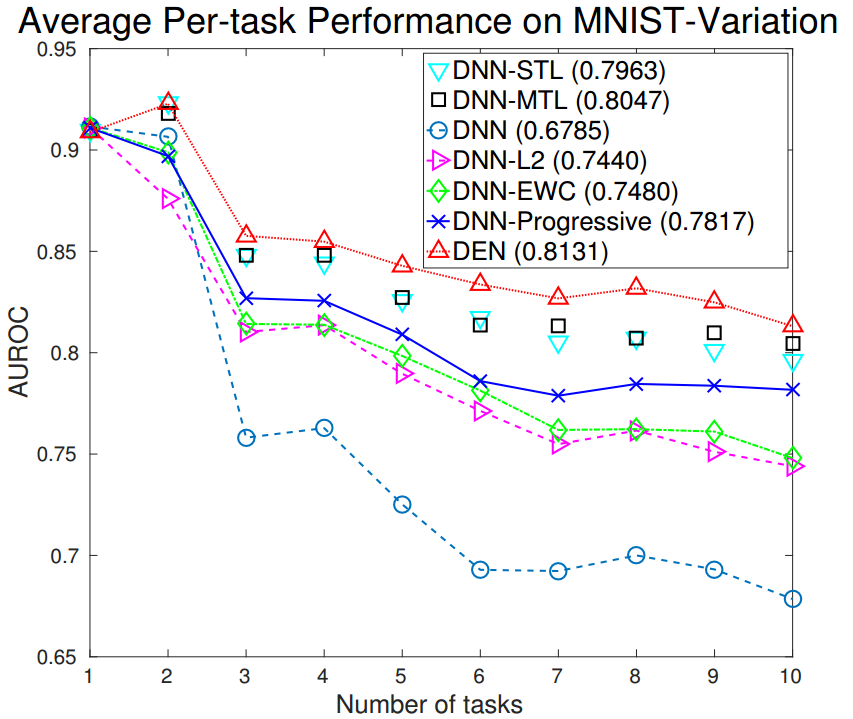
\includegraphics[width=\textwidth]{acc_them_den}
\end{minipage}
\hfill
\begin{minipage}{.49\textwidth}
    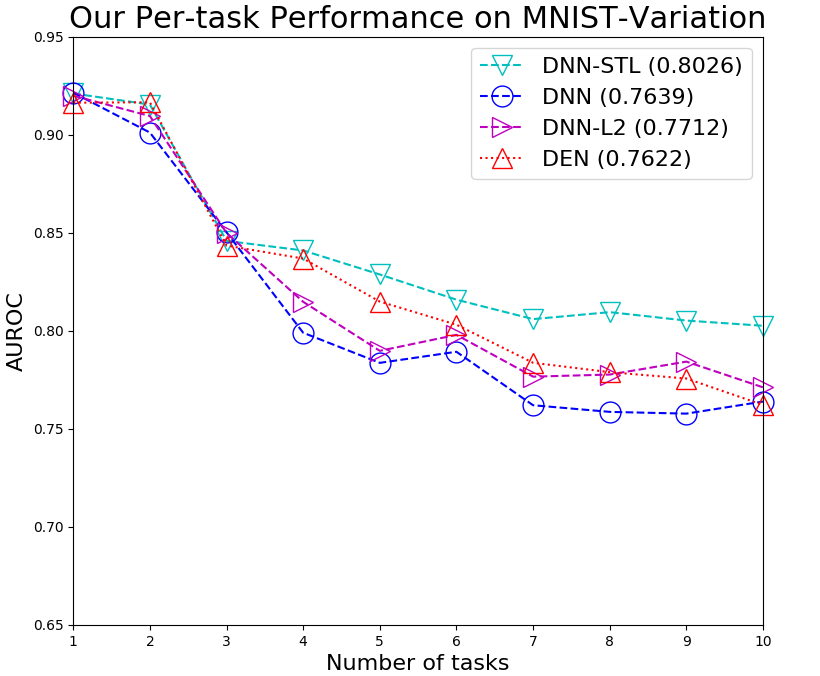
\includegraphics[width=\textwidth]{acc_us_den}
\end{minipage}
\end{center}
\end{posterbox}

\begin{posterbox}[name=discussion,column=2,below=TE]{Discussion}
This article proposes intuitive approaches on lifelong learning issues, but lacks detailed explanation of some keypoints.
\begin{itemize}
    \item Hyperparameters values undisclosed
    \item Network sparsity is not guaranteed, contrary to what is claimed
    \item Questionable design of duplication (different from released code)
    \item MNIST dataset seems inadequate to test performances of lifelong learning models
    \item Dubious evaluation metric
\end{itemize}

\end{posterbox}






\begin{posterbox}[name=refs,column=2,above=bottom]{References}
% In the last box, you will usually have a list of references
% The bibliography automatically adds the title "References", but
% this have been removed in the preamble

% use either ......
\bibliographystyle{plain}
\bibliography{poster}


% ...... or
%  \bibliographystyle{IEEEbib}
%  \bibliography{IEEEabrv,mybib,mybib2} 
\end{posterbox}

\end{poster}
\end{document}
